\documentclass[11pt,a4paper]{article}
\usepackage[utf8]{inputenc}
\usepackage{graphicx}
\usepackage{float}
\usepackage{amsmath}
\usepackage{amssymb}
\usepackage{geometry}
\usepackage{hyperref}
\usepackage{booktabs}
\usepackage{microtype}

\geometry{
    a4paper,
    total={170mm,257mm},
    left=20mm,
    top=20mm,
}

\hypersetup{
    colorlinks=true,
    linkcolor=blue,
    filecolor=magenta,      
    urlcolor=cyan,
    pdftitle={Action Recognition on miniUCF},
    pdfpagemode=FullScreen,
}

\title{\textbf{Action Recognition on miniUCF}}
\author{}
\date{\today}

\begin{document}

\maketitle

\section{Dataset Implementation}
Each task has its own dataset implementation because the two models require different temporal input formats.

For TSN, \texttt{TSN/dataset.py} samples one item from each temporal segment of a video. RGB input returns tensors shaped:
\begin{verbatim}
[segments, 3, height, width]
\end{verbatim}

Optical-flow input returns tensors shaped:
\begin{verbatim}
[segments, 14, height, width]
\end{verbatim}

The 14 flow channels come from stacking 7 consecutive \texttt{(flow\_x, flow\_y)} pairs. The TSN dataset uses 4 temporal segments.

For 3D ResNet, \texttt{3DResNet/dataset.py} samples contiguous RGB clips. Training uses a random temporal crop. Validation uses multi-view testing, where several clips are sampled from different temporal positions in the same video.

The 3D ResNet training tensor shape is:
\begin{verbatim}
[3, clip_length, 112, 112]
\end{verbatim}

The validation tensor shape is:
\begin{verbatim}
[num_views, 3, clip_length, 112, 112]
\end{verbatim}

\section{Task 1: Temporal Segment Network}

\begin{figure}[H]
    \centering
    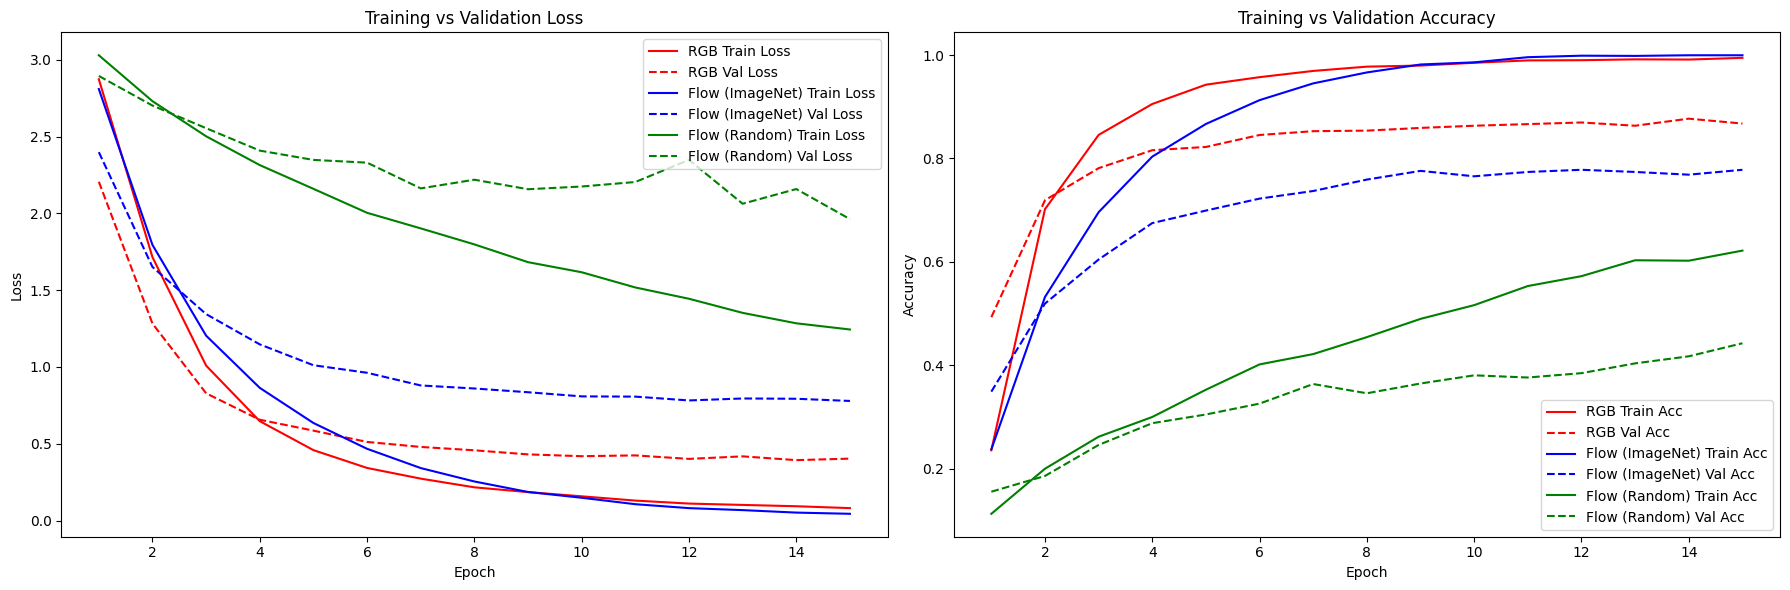
\includegraphics[width=0.85\textwidth]{Task1.png}
    \caption{Task 1 training curves}
    \label{fig:task1_curves}
\end{figure}

The RGB ImageNet model performs best overall, it reached higher accuracy than the Flow ImageNet model and earlier too.

The results show that ImageNet initialization is important for TSN, especially when the dataset is small. The RGB model converges fastest and generalizes best among the tested TSN settings. The optical-flow random model improves steadily so maybe it needs more epochs to converge but then we risk overfitting.

\section{Task 2: 3D ResNet-18}

Two initialization strategies are implemented:
\begin{itemize}
    \item Random PyTorch initialization
    \item Inflated ImageNet ResNet-18 initialization
\end{itemize}

For inflated initialization, each 2D convolution weight is copied along the temporal dimension and divided by the temporal kernel size:
\begin{verbatim}
[out, in, h, w] -> [out, in, t, h, w]
\end{verbatim}

The training data augmentation includes:
\begin{itemize}
    \item Temporal random cropping
    \item Spatial random cropping
    \item Random horizontal flipping
\end{itemize}

At validation time, the dataset performs 4-view temporal testing by default. The model predicts each view separately, then the validation loop averages the view logits to obtain one video-level prediction.

\begin{figure}[H]
    \centering
    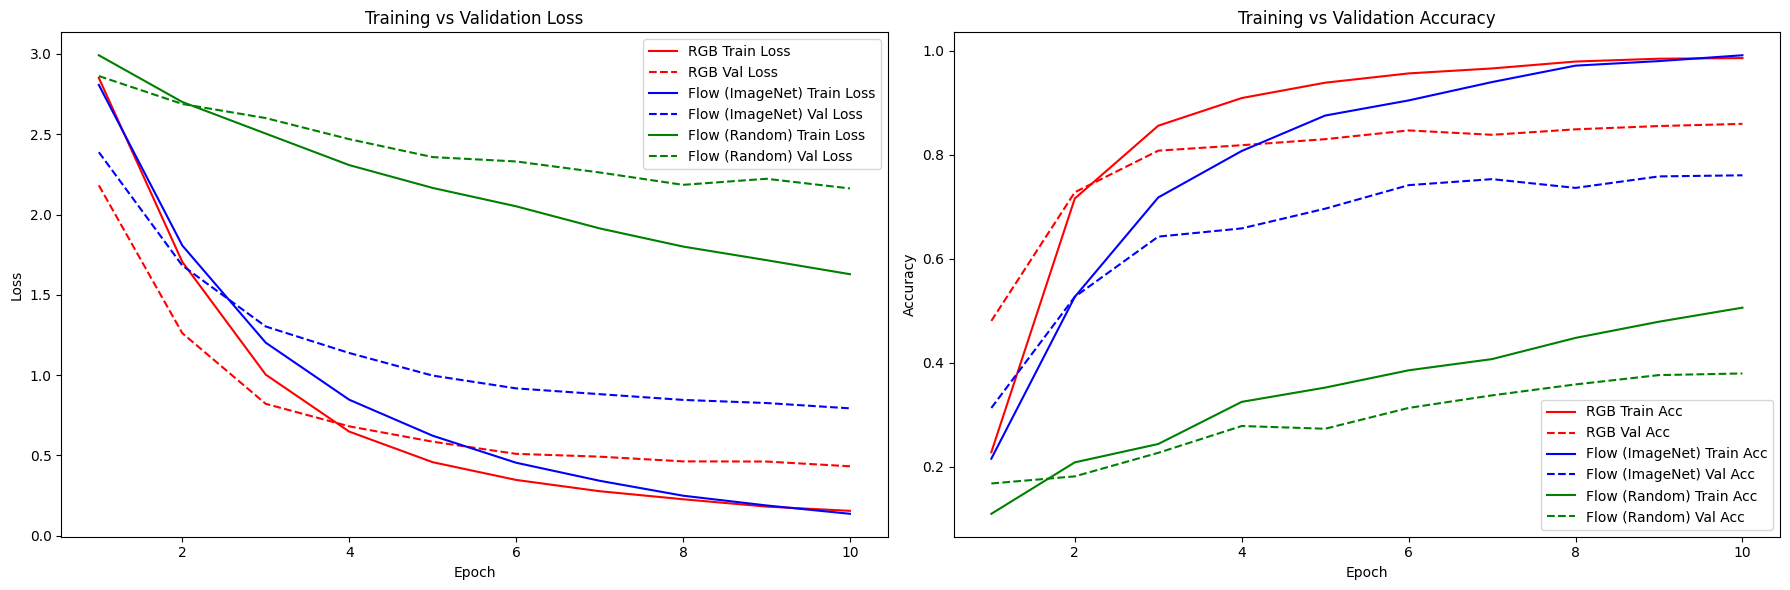
\includegraphics[width=0.85\textwidth]{Task2.png}
    \caption{Task 2 training curves}
    \label{fig:task2_curves}
\end{figure}

The ImageNet-inflated 3D ResNet clearly outperforms the randomly initialized 3D ResNet. After 5 epochs, the ImageNet-inflated model reaches about 0.78 validation accuracy, while the random model reaches about 0.45 validation accuracy. The validation loss of the initialized model drops steadily, while the random model's validation loss remains much higher and starts to flatten.

The curves also show some overfitting in the ImageNet-initialized 3D ResNet: training accuracy continues rising to about 0.96 while validation accuracy improves more slowly and saturates near 0.78. This is expected because 3D CNNs have high capacity and miniUCF is relatively small.

\end{document}
